\begin{frame}[fragile,label=authPtr1]{authenticated pointers (1)}
\begin{lstlisting}[language={},style=smaller]
some_function:
    authentication_code <- MAC(
        secret key, 
        return address
    )
    ... dangerous function code ...
    assert(authenication_code ==
        MAC(secret key, return addres))
    jump to return address
\end{lstlisting}
\end{frame}

\begin{frame}[fragile,label=authPtr2]{authenticated pointers (2)}
\begin{lstlisting}[language={},style=smaller]
some_function:
    authentication_code <- MAC(
        secret key,
        stack pointer, 
        return address
    )
    ... dangerous function code ...
    assert(authenication_code ==
        MAC(secret key, stack pointer, return address))
    jump to return address
\end{lstlisting}
\end{frame}


\begin{frame}[fragile,label=authPtr3]{authenticated pointers (3)}
\begin{lstlisting}[language={},style=smaller]
some_function:
    return address <- encode(
        secret key,
        stack pointer, 
        return address
    )
    ... dangerous function code ...
    return address <- decode_or_crash(
        secret key,
        stack pointer, 
        return address
    )
    jump to return address
\end{lstlisting}
\end{frame}

\begin{frame}[fragile,label=authPtr4]{authenticated pointers (4)}
\begin{lstlisting}[language={},style=smaller]
some_vtable[index] <- encrypt(
    secret key,
    label,
    address of some of function
)
... dangerous code ...
function pointer <- decrypt(
    secret key,
    label,
    object->vtable[index]
)
call function pointer
\end{lstlisting}
\end{frame}

\begin{frame}{ARM authenticated pointers}
    \begin{itemize}
    \item ARM64 implements this idea with:
    \vspace{.5cm}
    \item secret key kept in a special register (hard to leak to attacker)
    \item authentication code placed in upper pointer bits
        \begin{itemize}
        \item makes pointer temporarily invalid
        \item can't ``accidentally'' use authenticated pointer without verifying authentication code first
        \end{itemize}
    \end{itemize}
\end{frame}

\begin{frame}{authenticated pointer layout}
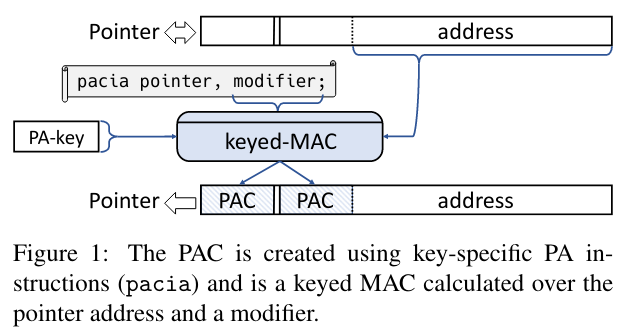
\includegraphics[width=\textwidth]{../cfi/arm-enc-ptr-fig}
\imagecredit{Liljestrand et al, ``PAC it up: Towards Pointer Integrity using ARM Pointer Authentication''}
\end{frame}

\begin{frame}{authentication keys}
    \begin{itemize}
    \item processes can have multiple authentication keys active
    \item easy to use separate keys for
        \begin{itemize}
        \item return address pointers
        \item function pointers
        \item any pointers to data
        \end{itemize}
    \item authentication keys are in special registers --- need OS to read/set
    \vspace{.5cm}
    \item also can ``mix'' in extra info like stack pointer
    \end{itemize}
\end{frame}

\begin{frame}{pointer authentication compiler support?}
    \begin{itemize}
    \item commonly enabled on ARM64 for return addreses
    \item known to be used more extensively on macOS X/iOS kernel
    \item proposals to use on Linux in global offset table, etc.
        \begin{itemize}
        \item GNU Linux linker option -z pac-plt; unclear if used `for real'
        \end{itemize}
    \end{itemize}
\end{frame}
